\documentclass{article}
\usepackage{graphicx}

\begin{document}
\section{LATR Optical Design}

The large aperture receiver is composed of an a array of 85 three lens cameras in an hexagonal packing. Each camera is made of three plano convex silicon lenses and a Lyot stop which reimages the primary. A silica prism is placed in front of the first lens to keep the camera axes parallel. The silica prism surface tilt and clocking is defined such that the chief ray of the center field of each camera lands at the focal plane in the center.

For the TMA, the surface of each lens $(z(r)$) is defined as a conic surface of revolution plus 8 polynomial terms in $r$, with $r$ measured from the center of the lens according to the equation\begin{equation}
	z(r) = \frac{cr^2}{1+\sqrt{1-(1+k)c^2r^2}} + \sum_{j=1}^{8} \alpha_{2j} r^{2j}
\end{equation}

where $c$ is the curvature (defined as $c=1/R$, with R is the radius of curvature), $k$ is the conic constant, and $\alpha_{k}$ are the even coefficients of the polynomial expansion. 

\begin{figure}
	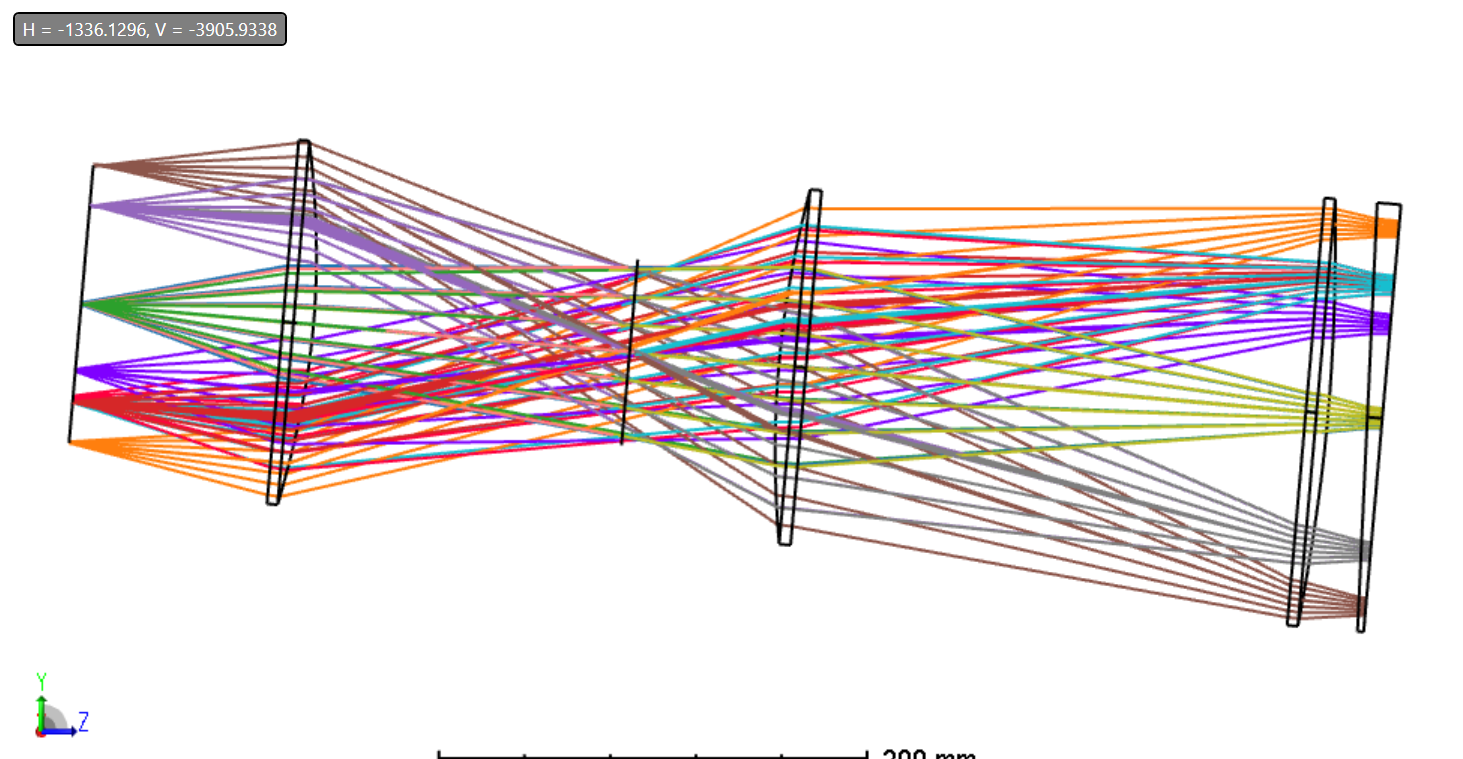
\includegraphics[width=0.48\textwidth]{TMP_cam1_layout.PNG}
	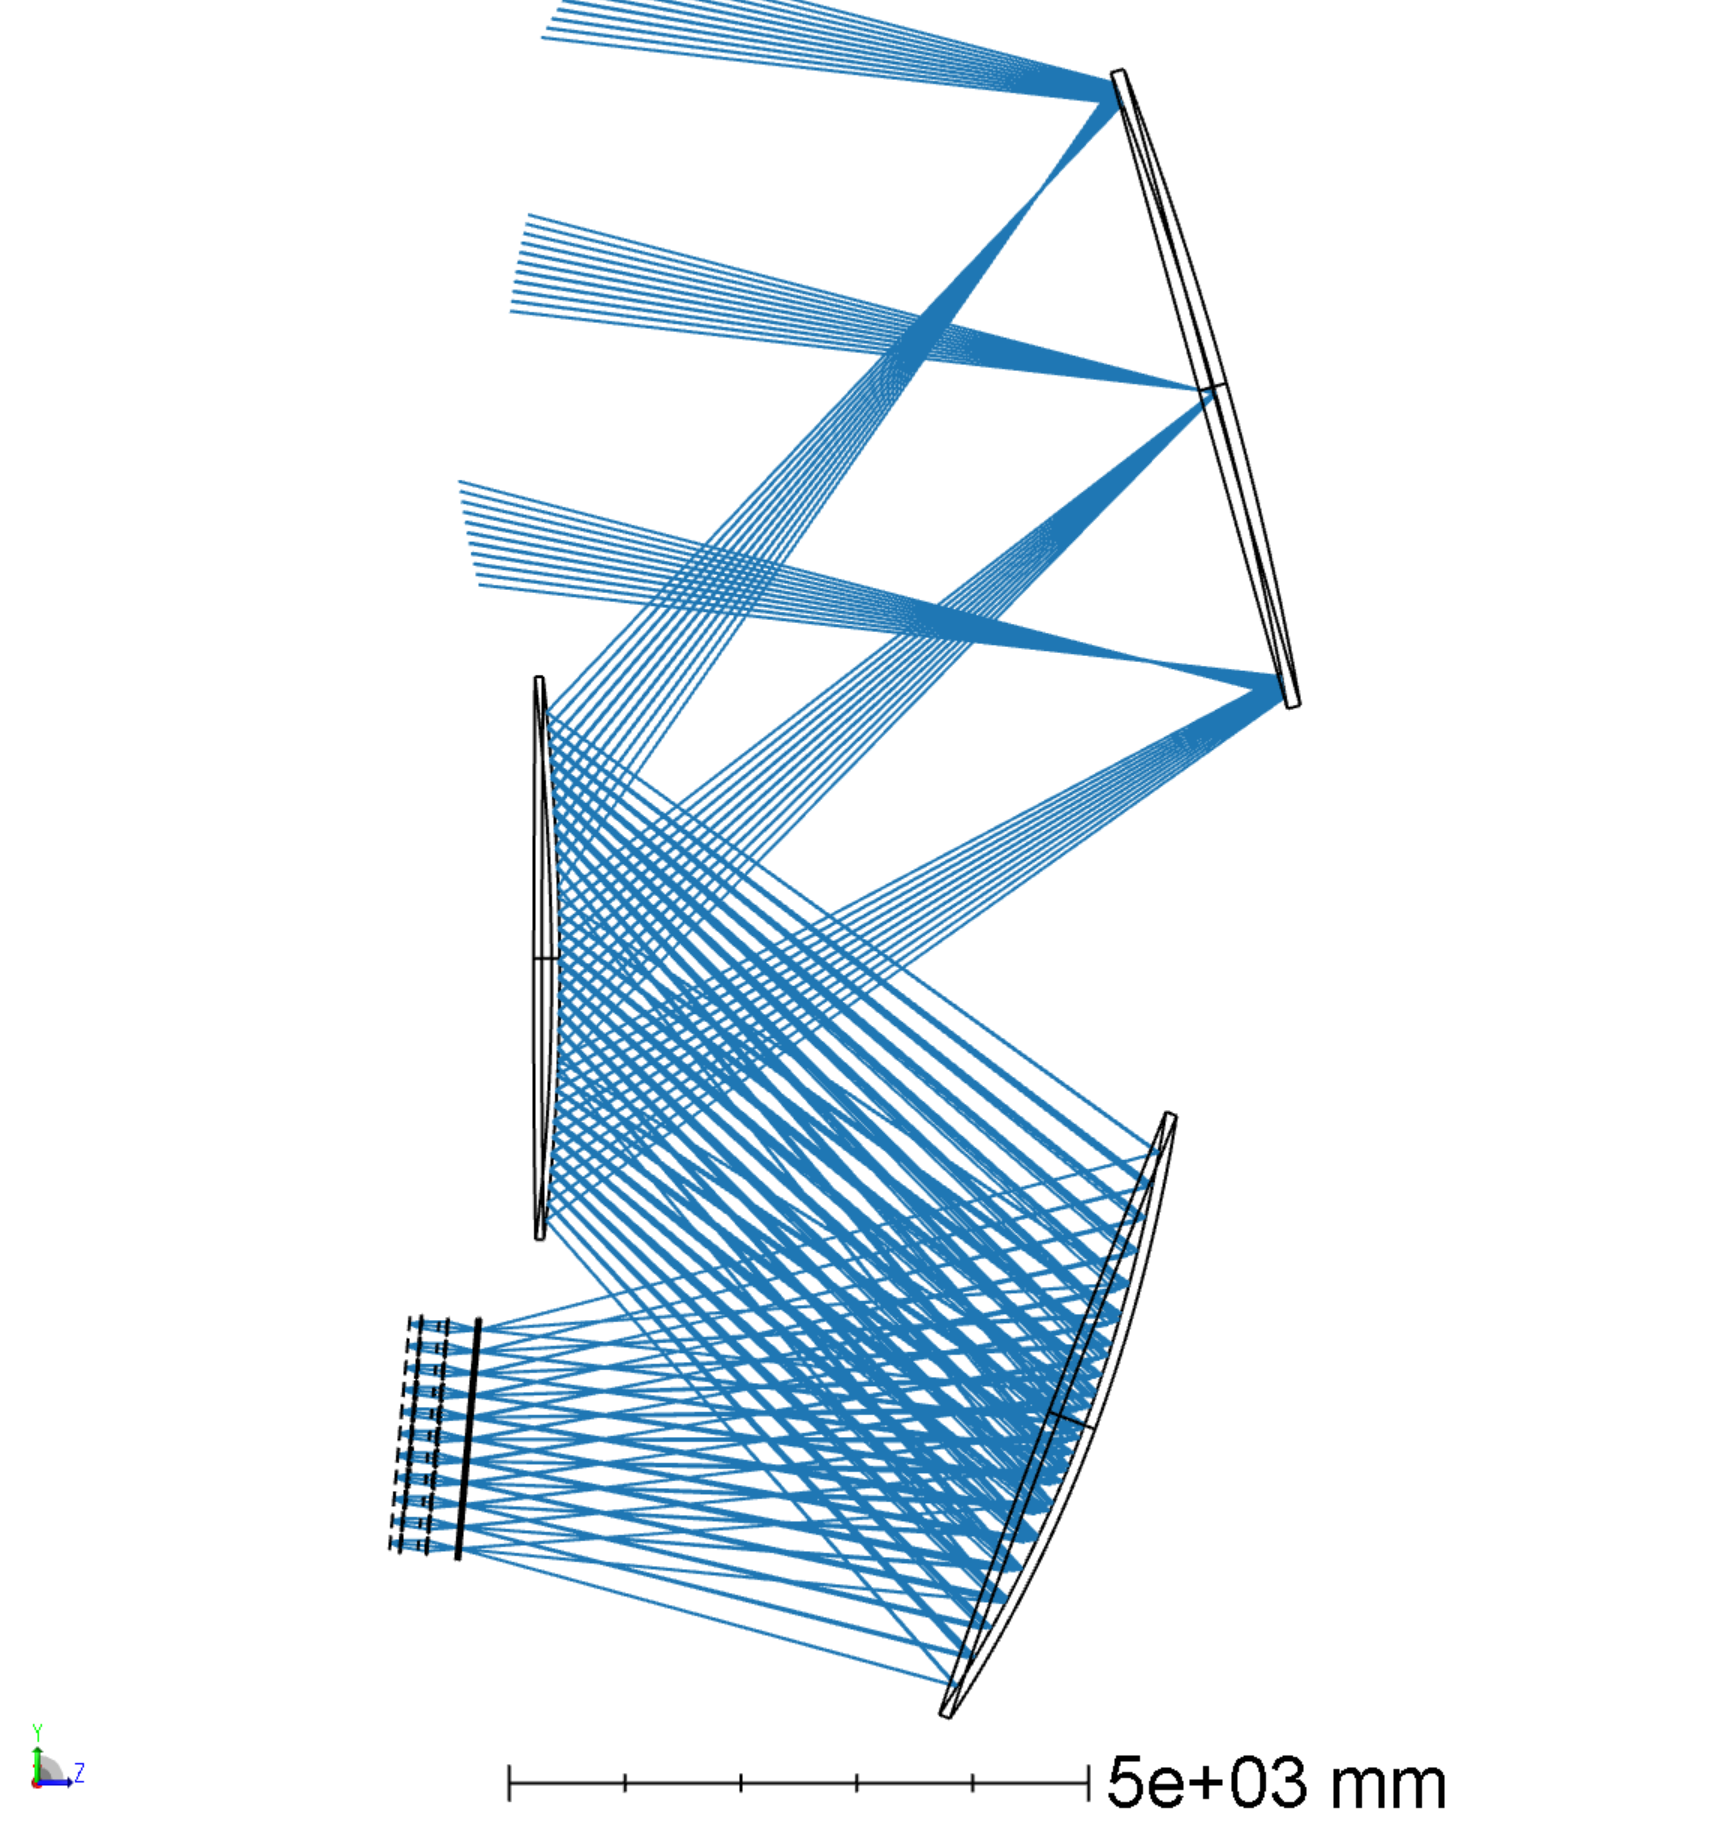
\includegraphics[width=0.48\textwidth]{TMP_3DLayout.png}
	
	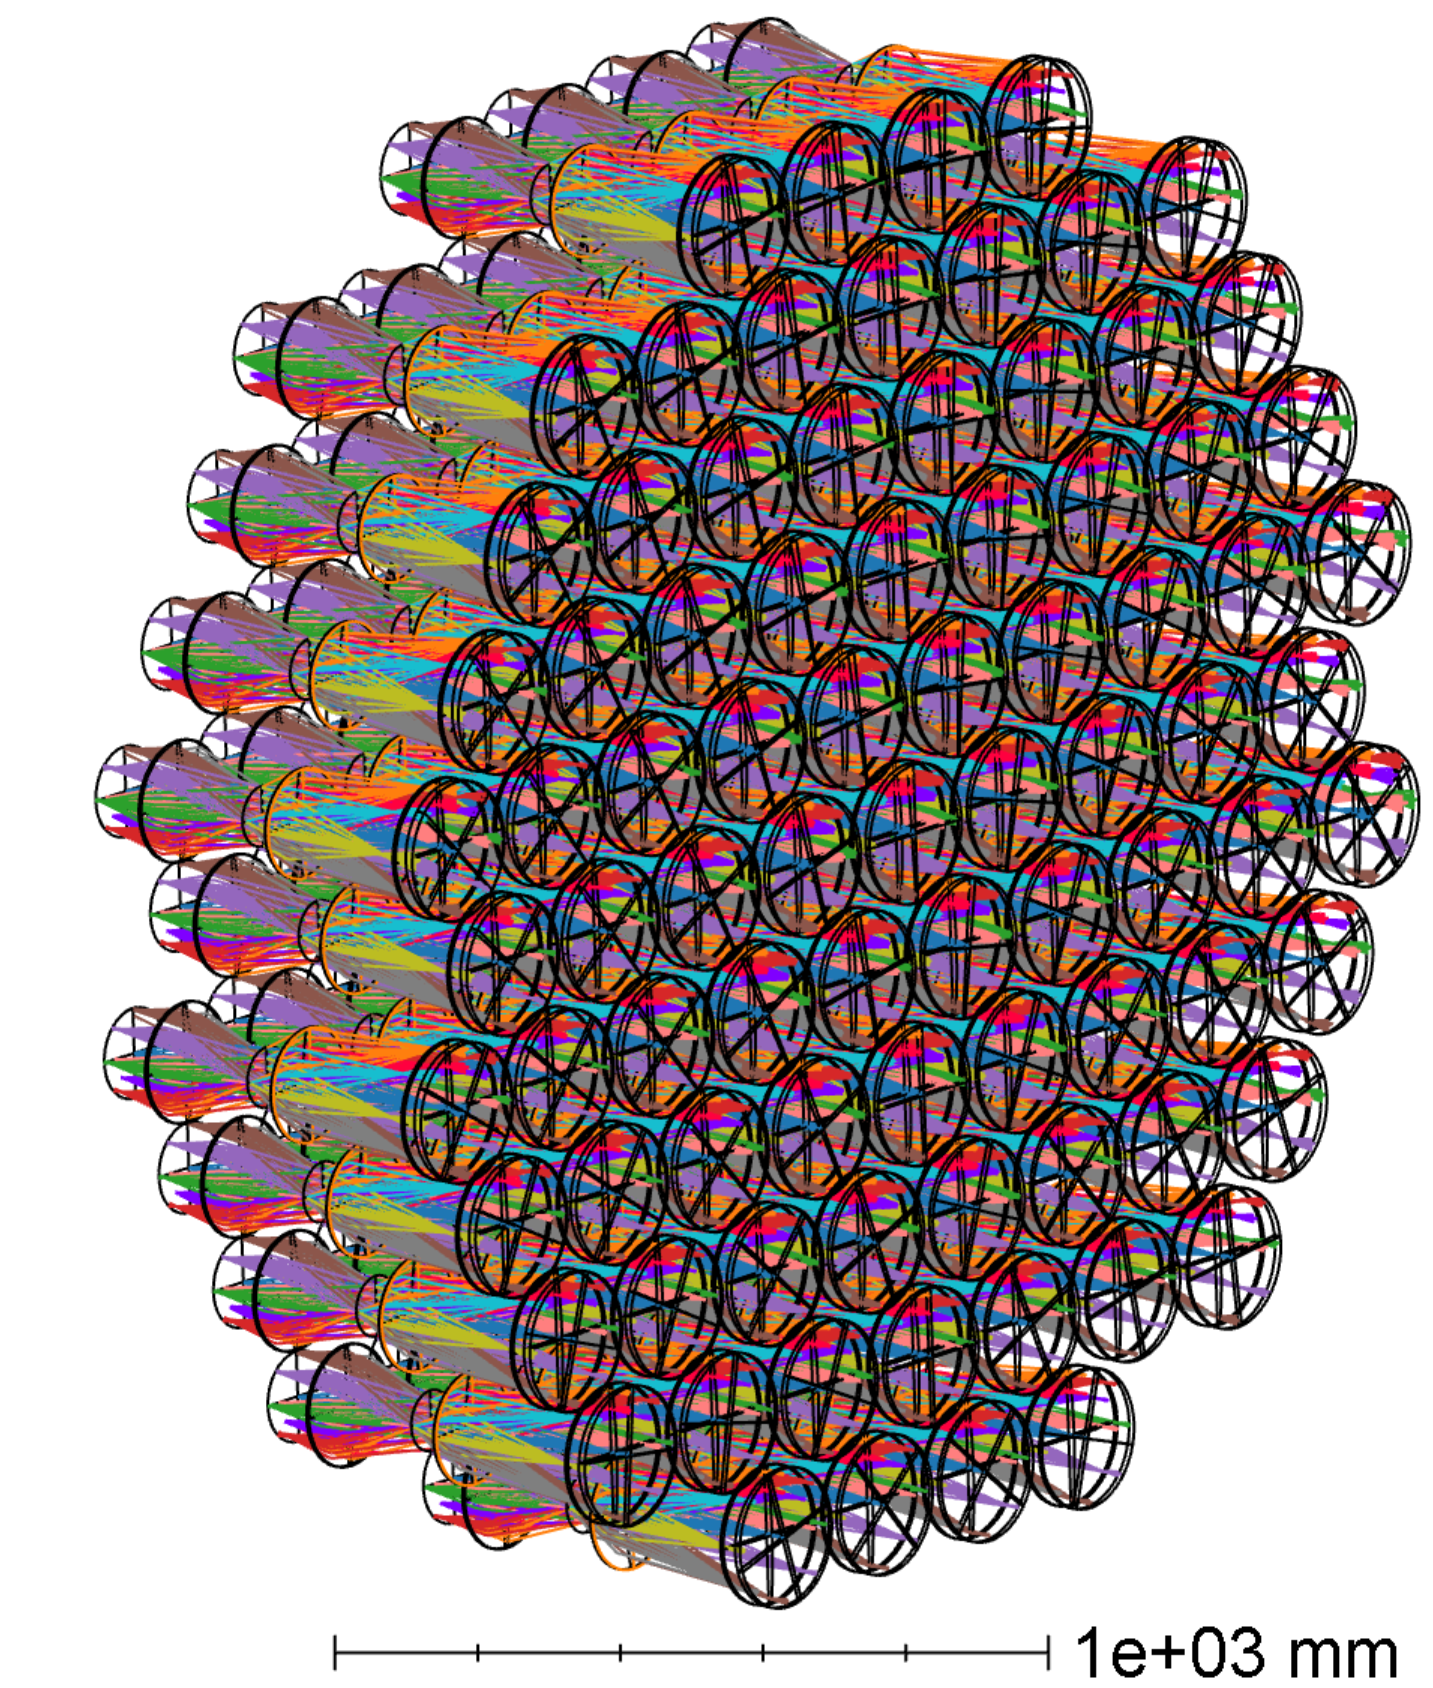
\includegraphics[width=0.48\textwidth]{TMP_cams.PNG}
\end{figure}

The CD camera lenses are composed of biconic lenses whith \begin{equation}
	z_{biconic} = \frac{c_x x^2 + c_y y^2}{1+ \sqrt{1-(1-k_x)c_x^2 x^2-(1+k_y)c_y^2y^2}} + \sum_{i=1}^{16} \alpha_i x^i + \sum_{j=1}^{16} \beta_j y^j 
\end{equation}

with curvatures given by  $c_x=\frac{1}{R_x}$ and $c_y=\frac{1}{R_y}$ and conic conic constants $k_{x,y}$




\end{document}